\documentclass[10pt, oneside]{article}
\usepackage{amsmath, amsthm, amssymb, calrsfs, wasysym, verbatim, bbm, color, graphics, geometry}
\usepackage{graphicx}
\graphicspath{ {./assets/} }
\geometry{tmargin=.75in, bmargin=.75in, lmargin=.75in, rmargin = .75in}

\newcommand{\R}{\mathbb{R}}
\newcommand{\C}{\mathbb{C}}
\newcommand{\Z}{\mathbb{Z}}
\newcommand{\N}{\mathbb{N}}
\newcommand{\Q}{\mathbb{Q}}
\newcommand{\Cdot}{\boldsymbol{\cdot}}

\newtheorem{thm}{Theorem}
\newtheorem{defn}{Definition}
\newtheorem{conv}{Convention}
\newtheorem{rem}{Remark}
\newtheorem{lem}{Lemma}
\newtheorem{cor}{Corollary}
\usepackage{biblatex} %Imports biblatex package
\addbibresource{reference.bib} %Import the bibliography file

\title{Summary Report: Inequality of opportunity, inequality of income and economic growth}
\author{Alejandro Ouslan}
\date{2025-04-16}

\begin{document}

\maketitle
\tableofcontents

\vspace{.25in}

\section{Summary}
This study \cite{aiyar2020inequality} looks to see if income inequality has an impact on growth. The authors of this paper found that
the is significant negative impact on the growth when the state poses more income inequality than those that poses less income inequality.
\section{Data sources}
The main database use is the Global Database on intergeneration Mobility from the World Bank \cite{gdim2018global}.

\section{Methodology}
\begin{equation}
	growth_{i \tau} = \rho y_{i \tau - 1} + (\theta_1 \theta_2 IM_i) \cdot GINI_{i \tau -1} + \Gamma X_{i \tau-1} + u_i + \gamma_{\tau} + \epsilon_{i \tau}
\end{equation}

where:
\begin{enumerate}
	\item $growth$ is the 55-year non overlapping average of real per capita gdp growth
	\item $i$ is the country
	\item $\tau$ is the time period starting in 1960
	\item $y$ is the log real GDP per capita
	\item $u_i$ and $\gamma_\tau$ denotes country fixed effects and period specific dummies
	\item
\end{enumerate}

The dataset consists of:
\begin{enumerate}
	\item $166$ countries
	\item spans from $1950$ to $2015$
	\item this includes $4437$ separate GINIS.
	\item $X$ is the matrix of covariates that are standard across-country
\end{enumerate}

\section{results}

\begin{figure}
	\centering
	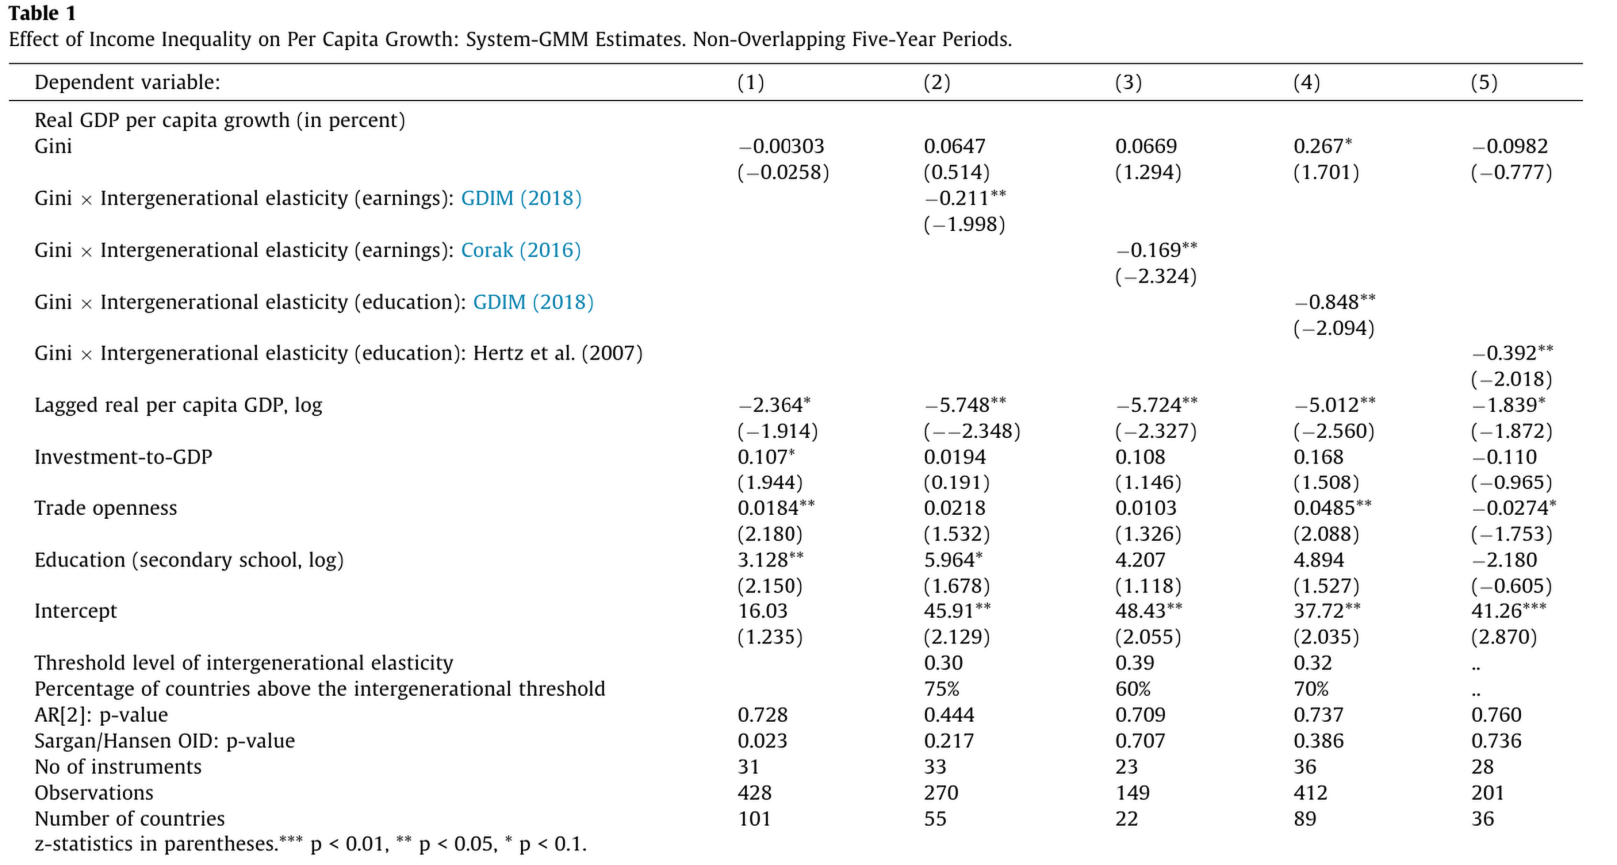
\includegraphics[width=\textwidth]{table_1.png}  % Adjust the width as needed
	\caption{Caption for Table 1}
\end{figure}

\begin{figure}
	\centering
	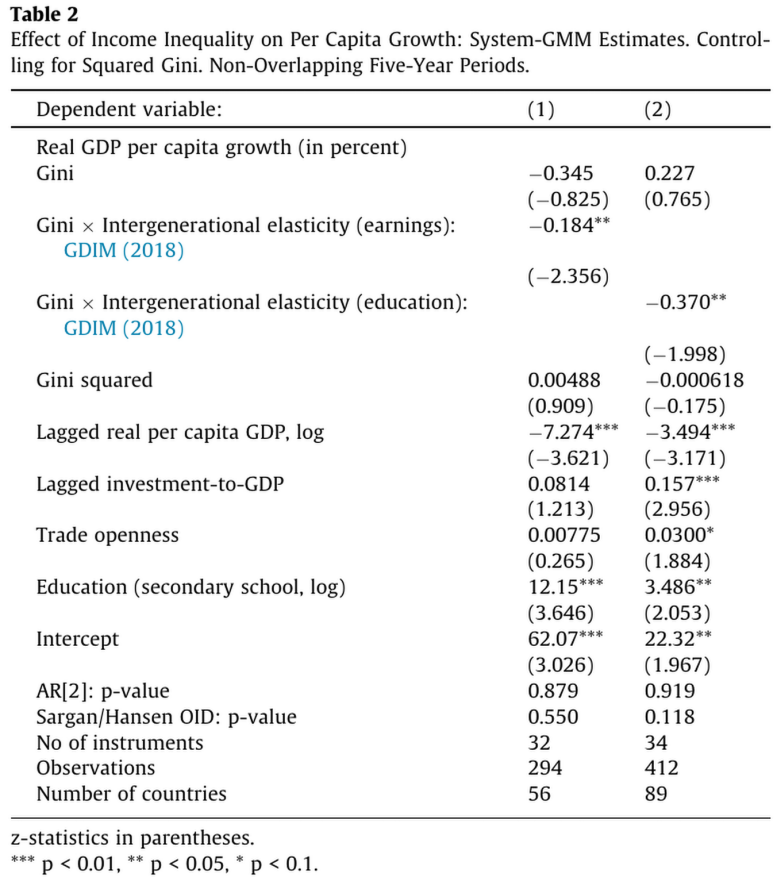
\includegraphics[width=\textwidth]{table_2.png}  % Adjust the width as needed
	\caption{Caption for Table 2}
\end{figure}

\section{Conclusions}

The main conclusions of this paper is that there is a negative relationship with income inequality on the countries growth. That is to say and increase
in income inequality of a particular country would be correlated with a decrease in the countries growth

\printbibliography
\end{document}
